\documentclass{uimppracticas}

%Permitir cabeceras y pie de páginas personalizados
\pagestyle{fancy}

%Path por defecto de las imágenes
\graphicspath{ {./images/} }

%Declarar formato de encabezado y pie de página de las páginas del documento
\fancypagestyle{doc}{
  %Pie de Página
  \footerpr{}{}{{\thepage} de \pageref{LastPage}}
}

%Declarar formato de encabezado y pie del título e indice
\fancypagestyle{titu}{%
  %Cabecera
  \headerpr{}{}{}
  %Pie de Página
  \footerpr{}{}{}
}

\appto\frontmatter{\pagestyle{titu}}
\appto\mainmatter{\pagestyle{doc}}

\begin{document}
	
%Comienzo formato título
\frontmatter

%Portada (Centrado todo)
\centeredtitle{./images/LogoUIMP.png}{Máster Universitario en Investigación en Inteligencia Artificial}{Curso 2020-2021}{Recuperación y extracción de información, \\ grafos y redes sociales}{Análisis y Visualización Básica de una Red Social con Gephi}

\begin{center}
\large \today
\end{center}

\vspace{40mm}

\begin{flushright}
 	{\bf Laura Rodríguez Navas}\\
 	\textbf{DNI:} 43630508Z\\
 	\textbf{e-mail:} \href{rodrigueznavas@posgrado.uimp.es}{rodrigueznavas@posgrado.uimp.es}
\end{flushright}

\newpage

%Índice
% \tableofcontents

% \newpage

%Comienzo formato documento general
\mainmatter

\setlength\parskip{2.5ex}

\section*{La Red}

La red \textit{Diseasome}\cite{Goh8685} seleccionada para realizar esta práctica, es una red no dirigida de trastornos y genes de diferentes enfermedades vinculadas por asociaciones conocidas entre trastornos y genes, que indican el origen genético común de muchas enfermedades. La red está formada por 526 enfermedades y 903 genes, donde los genes asociados con trastornos similares muestran una mayor probabilidad de interacciones físicas entre sus diagnósticos y una mayor similitud de perfiles de expresión para sus tratamientos, lo que respalda la existencia de distintos clústers funcionales específicos de cada enfermedad. 

El conjunto de datos de \textit{Diseasome} viene como un archivo \textit{.zip}, que se puede descargar \href{http://gephi.org/datasets/diseasome.gexf.zip}{aquí}. Que una vez se ha descargado y descomprimido, obtenemos un archivo \textit{.gexf}, un archivo de grafos. Importamos el archivo de grafos a \textit{Gephi}\cite{Gephi} y empezamos a probar diferentes opciones de visualización.

Después de probar diferentes visualizaciones nos decidimos por el algoritmo de distribución: \href{https://github.com/gephi/gephi/wiki/Fruchterman-Reingold}{Fruchterman Reingold}\cite{fruchterman1991graph} (en la ventana \textit{Distribución}). Para evitar que las componentes conexas queden fuera de la vista principal, fijamos el valor del parámetro \textit{Gravedad} a 20 y también marcamos las opciones \textit{Disuadir Hubs y/o Evitar el solapamiento}. Esto convertirá nuestra visualización de la red en un círculo y colocará la red alrededor de una misma área (ver Figura \ref{completa_negro_FR}). 

\begin{figure}[H]
	\centering
	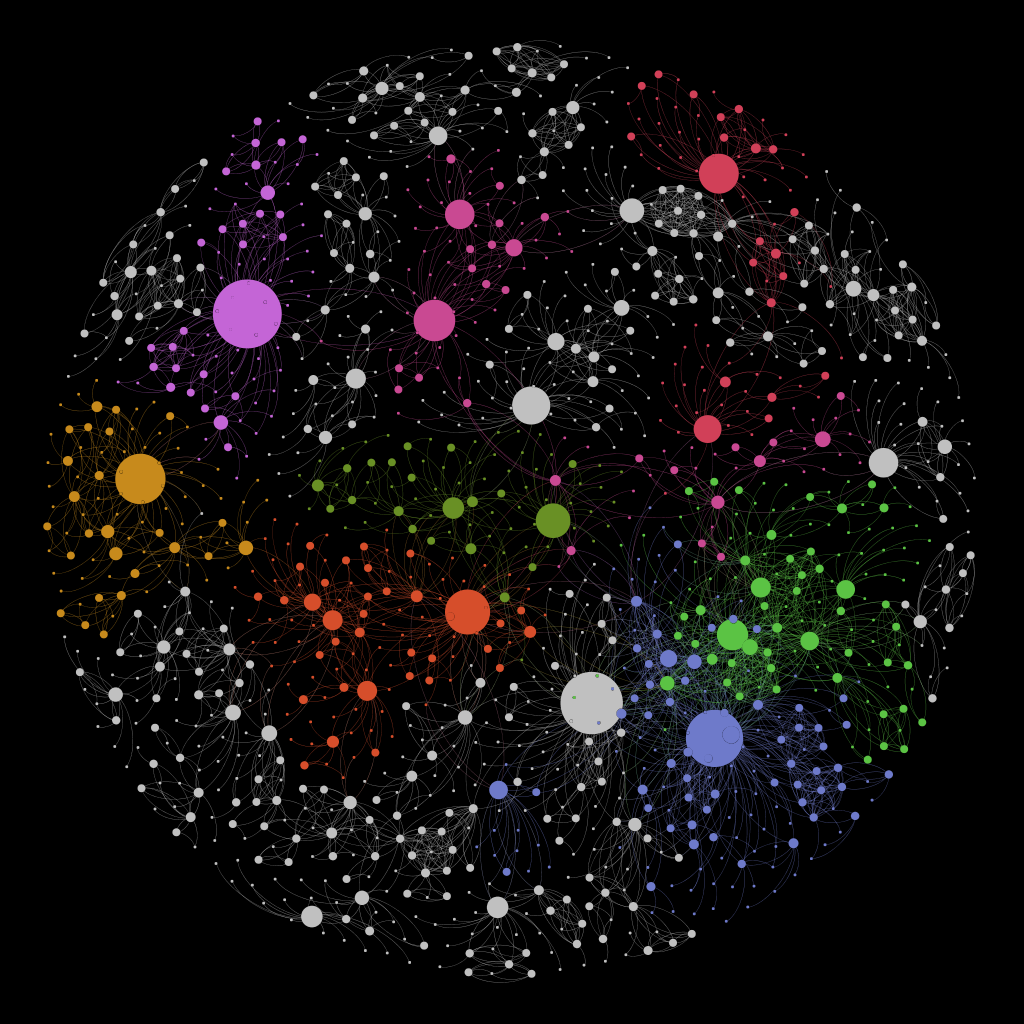
\includegraphics[width=0.6\textwidth]{images/completa_negro_FR}
	\caption{Red completa sobre un fondo negro sin etiquetas.}
	\label{completa_negro_FR}
\end{figure}

De una primera visualización pasamos a la detección de comunidades para colorear los clústers de la red. \textit{Gephi} implementa el método de \href{http://perso.uclouvain.be/vincent.blondel/research/louvain.html}{Louvain}\cite{Blondel2008} para la detección de comunidades (disponible en el panel de \textit{Estadísticas}). Para ello, damos clic en ejecutar \textit{Modularidad} y veremos como el algoritmo de detección de comunidades nos ha creado un nuevo parámetro de particionamiento llamado \textit{Modularity Class}. Si seleccionamos este nuevo parámetro podremos observar las comunidades encontradas y si finalmente pulsamos \textit{Aplicar} colorearemos los nodos según las comunidades encontradas. Esto hace que la visualización sea más colorida y se vea bien donde se encuentra cada comunidad. También añadimos etiquetas a los nodos (ver Figura \ref{completa_FR_labels}). 

\begin{figure}[H]
	\centering
	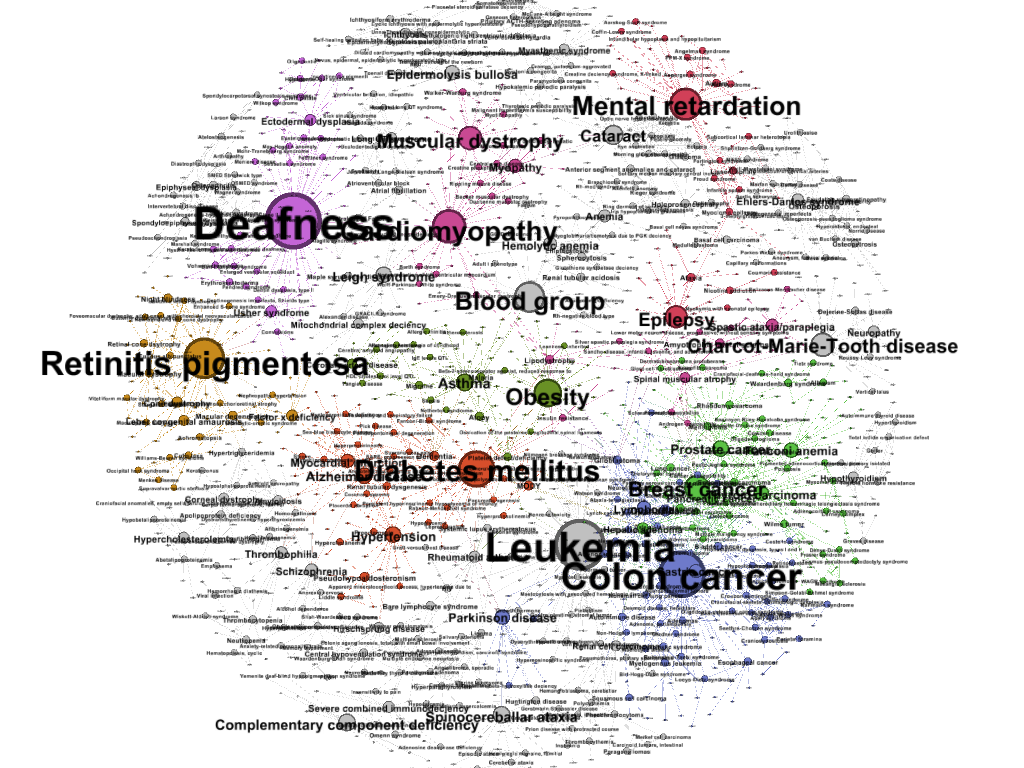
\includegraphics[width=0.85\textwidth]{images/completa_FR_labels}
	\caption{Red completa sobre un fondo blanco con etiquetas.}
	\label{completa_FR_labels}
\end{figure}

Como podemos observar en la Figura \ref{completa_FR_labels}, las diferentes comunidades están agrupadas por colores. El tamaño de las etiquetas depende del tamaño del nodo. Está claro que los cánceres son la enfermedad más dominante de todas, siendo una de las enfermedades más comunes en comparación con otras enfermedades que existen en la actualidad. Un dato curioso es que la sordera es la enfermedad que se lleva la mayor porción. También vemos otros clústers además de los cánceres, como la diabetes, la salud mental, etc. Se da la propiedad libre de escala (\textit{scale-free}), muy común en redes reales, porque muchos nodos de la red poseen un gran número de enlaces a otros nodos.

\section*{Análisis Básico de la Red}

Como pudimos observar en la sección anterior, la red parece demasiado compleja para analizarla visualmente, así que para los primeros pasos del análisis de la red, comenzamos por anotar los valores de las medidas globales básicas: el número de nodos ($N$) y el número de enlaces ($L$), que aparecen directamente en la ventana \textit{Contexto}. El número de nodos de la red es igual a 1419 y el número de enlaces es igual a 3926. Además calculamos manualmente el número máximo de enlaces $L_{max}$.

\begin{center}
	$L_{max} = \frac{N\,*\,(N-1)}{2} = \frac{1419\,*\,(1419-1)}{2} = 1006071$
\end{center}

Posteriormente calculamos otra medida global, el grado medio <k>, ejecutando la opción correspondiente en la ventana \textit{Estadísticas}. El valor del grado medio <k> es igual a 5,533, es decir, que cada trastorno de la red está conectado con 5 genes en media. Al realizar el cálculo del grado medio <k>, también obtenemos la distribución de grados de la red completa (ver Figura \ref{degree-distribution}).

\begin{figure}[H]
	\centering
	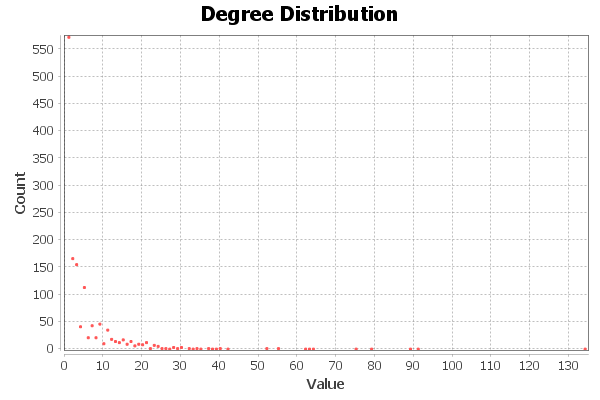
\includegraphics[width=0.55\textwidth]{images/degree-distribution}
	\caption{Distribución de grados de la red completa.}
	\label{degree-distribution}
\end{figure}

Existen algunas enfermedades fuertemente conectadas (\textit{hubs}), la mayor con grado 135. Concretamente 10 enfermedades tienen más de 50 variaciones de genes.

La opción \textit{Densidad} de grafo mide la relación entre el número de enlaces ($L$) y el número máximo de enlaces ($L_{max}$). Ejecutamos la opción y vemos que su valor es igual a 0,004 (valor cercano a 0, densidad mínima). Esto nos indica que el grafo es un grafo disperso, el número de enlaces ($L$) no es cercano al número de máximo de enlaces ($L_{max}$). 

A continuación, ejecutamos la opción \textit{Coeficiente medio de clustering <C>} para obtener la medida del mismo nombre. El valor del coeficiente medio de clustering es igual a 0,819. Es un valor muy alto que nos indica un grado muy significativo de clustering local. Al realizar el cálculo del coeficiente medio de clustering también obtenemos la distribución de coeficientes de clustering de la red completa (ver Figura \ref{clustering-coefficient}), donde vemos que el coeficiente de clustering es mucho mayor en los nodos poco conectados que en los nodos más conectados (\textit{hubs}). En este caso, los nodos de grado bajo se sitúan en vecindarios localmente densos y viceversa como consecuencia de la jerarquía de la red.

\begin{figure}[H]
	\centering
	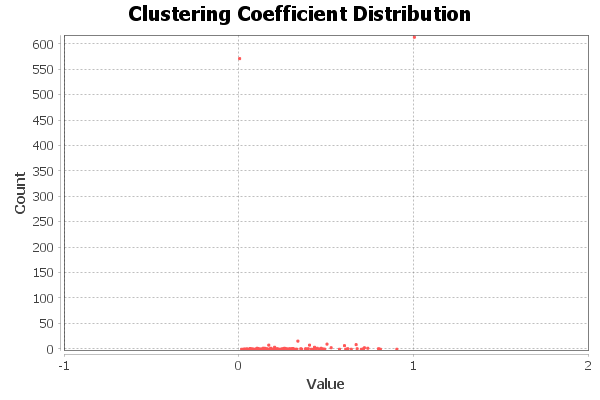
\includegraphics[width=0.55\textwidth]{images/clustering-coefficient}
	\caption{Distribución de coeficientes de clustering de la red completa.}
	\label{clustering-coefficient}
\end{figure}

Ahora, pasamos a analizar la conectividad de la red. En primer lugar, obtenemos el número de componentes conexas ejecutando la opción \textit{Componentes conexos} (disponible en el panel de \textit{Estadísticas}). Vemos  que el número de componentes conexas es igual a 1. En este caso, como solo tenemos una componente conexa, determinamos que la componente gigante de la red es la red completa actual.

Finalmente, calculamos las medidas globales restantes (diámetro $d_{max}$ y distancia media <d>) ejecutando la opción correspondiente al \textit{Diámetro de la red} en la ventana {Estadísticas}. El valor del diámetro ($d_{max}$) es igual a 15. Viendo la red (ver Figura \ref{completa_FR_labels}), pensaríamos que hay variaciones grandes en las distancias entre los nodos pero la red tiene una distancia media baja (<d> = 6,783). El cálculo del diámetro también nos proporciona los valores de las tres medidas de centralidad (intermediación, cercanía y excentricidad), que podemos observar en las figuras \ref{Betweenness-Centrality-Distribution}, \ref{Closeness-Centrality-Distribution} y \ref{Eccentricity-Distribution}.

\begin{figure}[H]
	\centering
	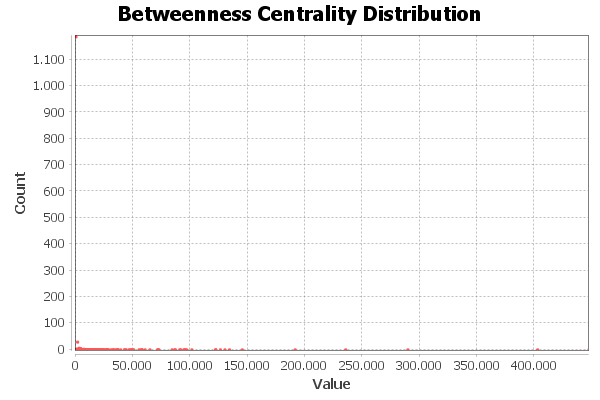
\includegraphics[width=0.55\textwidth]{images/Betweenness-Centrality-Distribution}
	\caption{Centralidad de intermediación no normalizada de la red completa.}
	\label{Betweenness-Centrality-Distribution}
\end{figure}

\begin{figure}[H]
	\centering
	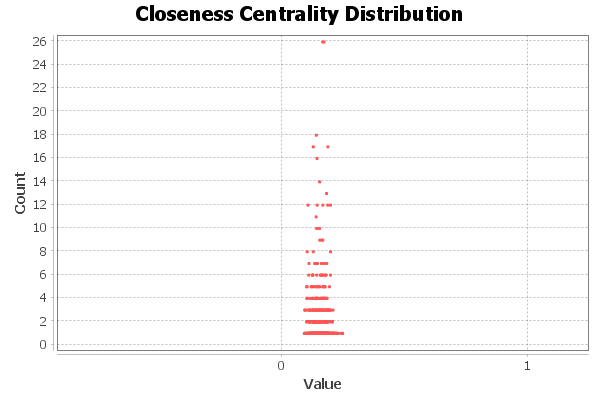
\includegraphics[width=0.55\textwidth]{images/Closeness-Centrality-Distribution}
	\caption{Centralidad de cercanía no normalizada de la red completa.}
	\label{Closeness-Centrality-Distribution}
\end{figure}

Observando la figura anterior parece que se de la propiedad de mundos pequeños (\textit{small-world}). La mayoría de los nodos no son vecinos entre sí, y sin embargo la mayoría de los nodos pueden ser alcanzados desde cualquier nodo origen a través de un número relativamente corto de saltos entre ellos. También observamos que no existen distancias largas en la red.

\begin{figure}[H]
	\centering
	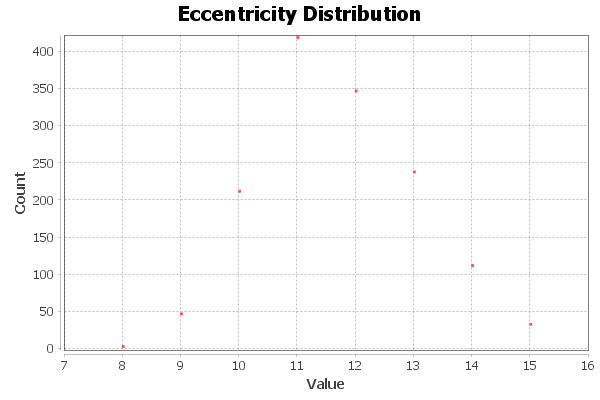
\includegraphics[width=0.55\textwidth]{images/Eccentricity-Distribution}
	\caption{Centralidad de excentricidad no normalizada de la red completa.}
	\label{Eccentricity-Distribution}
\end{figure}

A continuación, mostramos la tabla que resume los valores de las medidas calculadas anteriormente (ver fichero \textit{MedidasRedesPracticaParteI-1.xlsx} para observar la tabla en formato Excel).

\begin{table}[H]
	\centering
	\begin{tabular}{|l|r|}
		\hline
		\textbf{Medida}                                            & \textbf{Valor} \\ \hline\hline
		Número de nodos N                                          & 1419           \\ \hline
		Número de enlaces L                                        & 3926           \\ \hline
		Número máximo de enlaces Lmax                              & 1006071        \\ \hline
		Densidad del grafo L/Lmax                                  & 0.004          \\ \hline
		Grado medio \textless{}k\textgreater{}                     & 5.533          \\ \hline
		Diámetro dmax                                              & 15             \\ \hline
		Distancia media d                                          & 6.783          \\ \hline
		Coeficiente medio de clustering \textless{}C\textgreater{} & 0.819          \\ \hline
		Número de componentes conexas                              & 1              \\ \hline
		Número de nodos componente gigante                         & 1419           \\ \hline
		Número de aristas componente gigante                       & 3926           \\ \hline
	\end{tabular}
	\caption{Tabla con los valores de las medidas estudiadas.}
	\label{tabla}
\end{table}

En la siguiente sección de la práctica empleamos la medidas de centralidad calculadas.

\newpage

\section*{Estudio de la Centralidad de los Actores}

En esta sección se realiza un pequeño análisis de redes sociales sobre nuestra red basado en las medidas de centralidad. El análisis determina los 5 actores principales de la red mediante las medidas de centralidad de grado, intermediación, cercanía y vector propio.

Los valores de tres de estas medidas (grado, intermediación y cercanía) ya están calculados en los pasos que se han realizado en la sección anterior. La centralidad de grado (no normalizada) se generó al calcular el \textit{Grado medio <k>} en la ventana \textit{Estadísticas}. Las medidas de centralidad de intermediación y cercanía (no normalizadas) se generaron con la opción \textit{Diámetro de la red}. En este caso, las volvemos a calcular para obtener las medidas normalizadas con el checkbox \textit{Normalizar centralidades en el rango [0,1]}.

\begin{figure}[H]
	\centering
	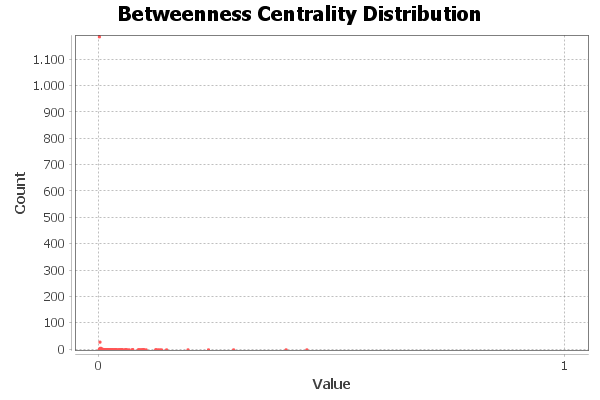
\includegraphics[width=0.6\textwidth]{images/Betweenness-Centrality-Distribution-Norm}
	\caption{Centralidad de intermediación normalizada de la red completa.}
	\label{Betweenness-Centrality-Distribution-Norm}
\end{figure}

\begin{figure}[H]
	\centering
	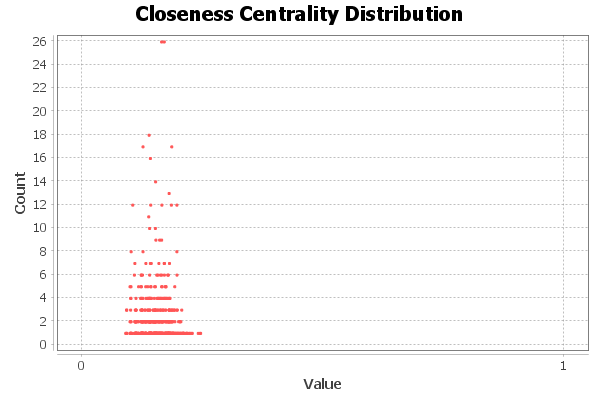
\includegraphics[width=0.6\textwidth]{images/Closeness-Centrality-Distribution-Norm}
	\caption{Centralidad de cercanía normalizada de la red completa.}
	\label{Closeness-Centrality-Distribution-Norm}
\end{figure}

Finalmente, calculamos la centralidad de vector propio que se calcula en la opción del menú \textit{Estadísticas} del mismo nombre (ver Figura \ref{Eigenvector-Centrality}).

\begin{figure}[H]
	\centering
	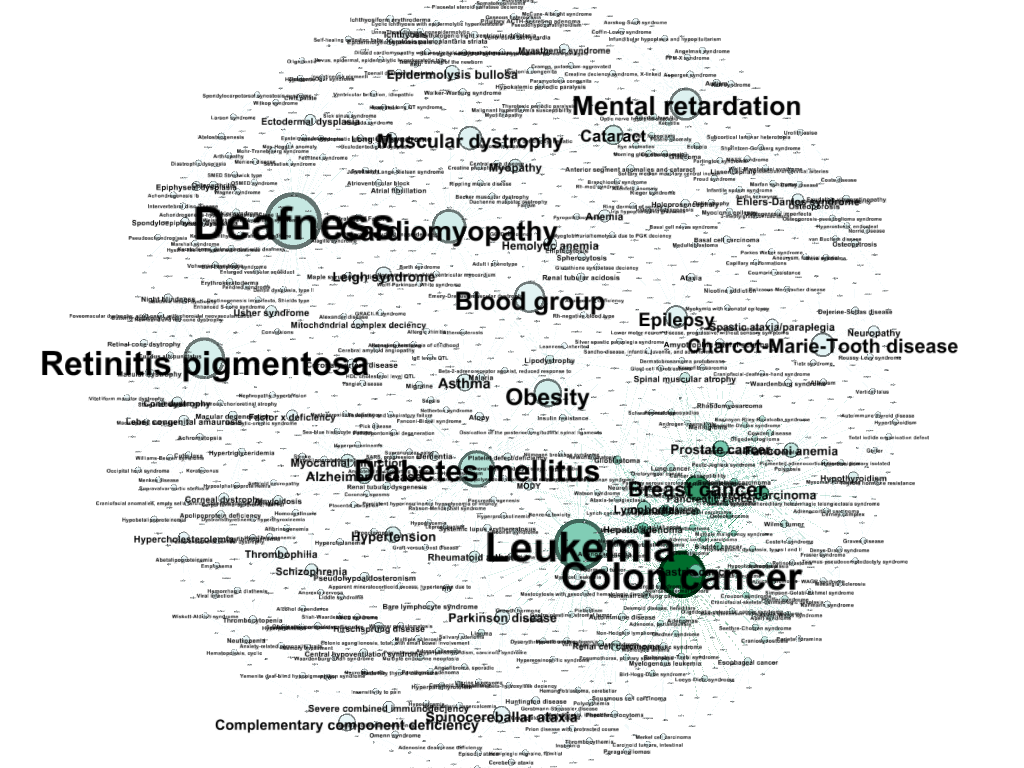
\includegraphics[width=0.6\textwidth]{images/Eigenvector-Centrality}
	\caption{Centralidad de vector propio de la red completa.}
	\label{Eigenvector-Centrality}
\end{figure}

Una vez ejecutadas las opciones de menú correspondientes, los valores de centralidad de cada nodo pueden visualizarse en la tabla \textit{Nodos} de la pestaña \textit{Tabla de datos}, junto con el resto de la información asociada a cada nodo. A continuación, anotamos los nombres de los 5 actores con mejor valor para cada una de las cuatro medidas anteriores, así como el valor de la medida en cada caso y los almacenamos en la tabla siguiente:

\begin{table}[H]
	\centering
	\begin{tabular}{ |c|c|c|c| } 
		\hline
		\thead{\textbf{Centralidad de} \\ \textbf{Grado}} & \thead{\textbf{Centralidad de} \\ \textbf{Intermediación}} & 	\thead{\textbf{Centralidad de } \\ \textbf{Cercanía}} & \thead{\textbf{Centralidad de } \\ \textbf{Vector propio}} \\ 
		\hline
		\thead{Colon Cancer \\ 134} & \thead{Cardiomyopathy \\ 0.445069}  & \thead{Lipodystrophy \\ 0.245414} & \thead{Colon cancer \\ 1.000000} \\ 
		\hline
		\thead{Deafness \\ 91} & \thead{Lipodystrophy \\ 0.400534} & \thead{Diabetes mellitus \\ 0.244272} & \thead{Breast cancer \\ 0.731462} \\ 
		\hline
		\thead{Leukemia \\ 89} & \thead{Diabetes mellitus \\ 0.28795} & \thead{Glioblastoma \\ 0.240402} & \thead{Thyroid carcinoma \\ 0.577893} \\ 
		\hline
		\thead{Breast Cancer \\ 79} & \thead{Glioblastoma \\ 0.234041} & \thead{Obesity \\ 0.228084} & \thead{Pancreatic cancer \\ 0.557891} \\ 
		\hline
		\thead{Diabetes mellitus \\ 75} & \thead{Deafness \\ 0.19061} & \thead{Cardiomyopathy \\ 0.226771} & \thead{Gastric cancer \\ 0.479706} \\ 
		\hline 
	\end{tabular}
	\caption{Los 5 actores con mejor valor por medida de centralidad.}
\end{table}

Los 5 actores mas importantes de la red desde una perspectiva global en función de los valores de las medidas de centralidad pertenecen a cánceres, diabetes, sordera, cardiopatías, VIH y obesidad. Aunque las centralidades de grado no tienen en cuenta la estructura global de la red, también las analizaremos ya que son medidas importantes.

\begin{itemize}
	\item Los cánceres tienen una alta centralidad de grado. Una alta centralidad de grado nos indica que son los actores con más enlaces que conectan con otros nodos. Si solo nos fijáramos en esta medida, los cánceres serian los actores más centrales. Pero, como no nos podemos quedar con una sola medida, analizamos también porque el clúster de cánceres tiene una alta centralidad de vector propio (los 5 actores pertenecen a este clúster). Sabemos que la centralidad de vector propio se basa en que la centralidad de un nodo concreto depende de cómo de centrales sean sus vecinos (prominencia).
	\item La sordera también tiene una alta centralidad de grado. Muchas personas en el mundo padecen sordera. También tiene una alta centralidad de intermediación.
	\item Las cardiopatías tienen una alta centralidad de intermediación. También tiene una alta centralidad de cercanía.
	\item El VIH y la diabetes tienen una alta centralidad de cercanía.
\end{itemize}

\newpage

\section*{Visualizaciones y Gráficos adicionales}

\begin{figure}[H]
	\centering
	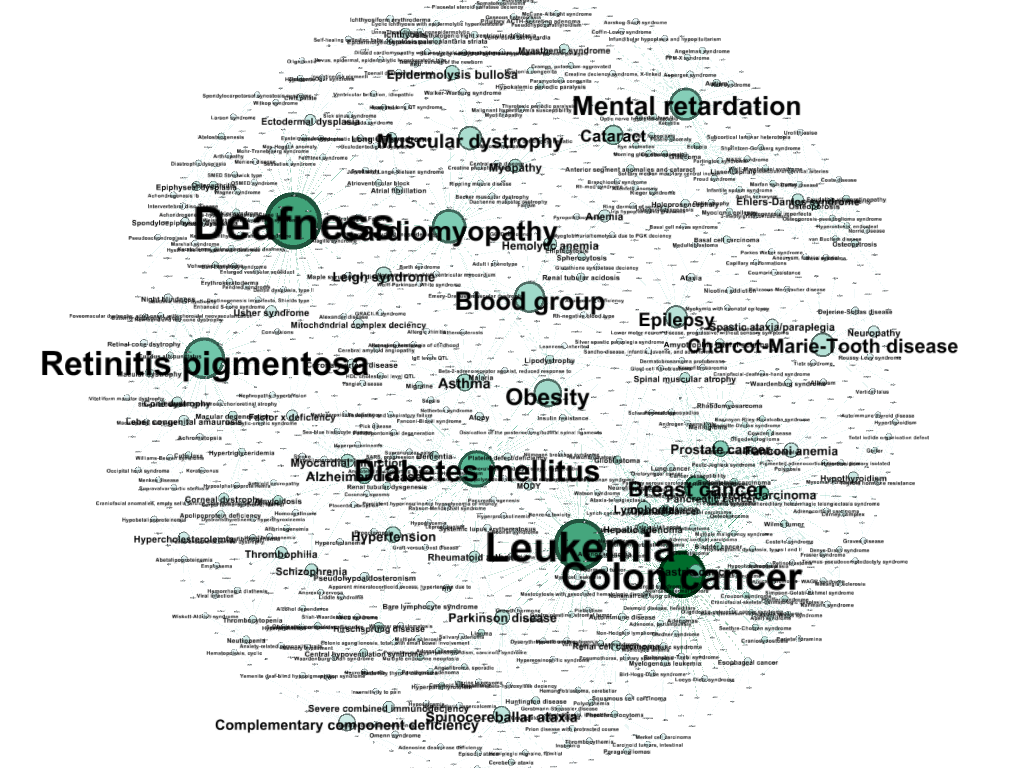
\includegraphics[width=0.75\textwidth]{images/Grado-Centrality}
	\caption{Centralidad de grado de la red completa.}
	\label{Grado-Centrality}
\end{figure}

\begin{figure}[H]
	\centering
	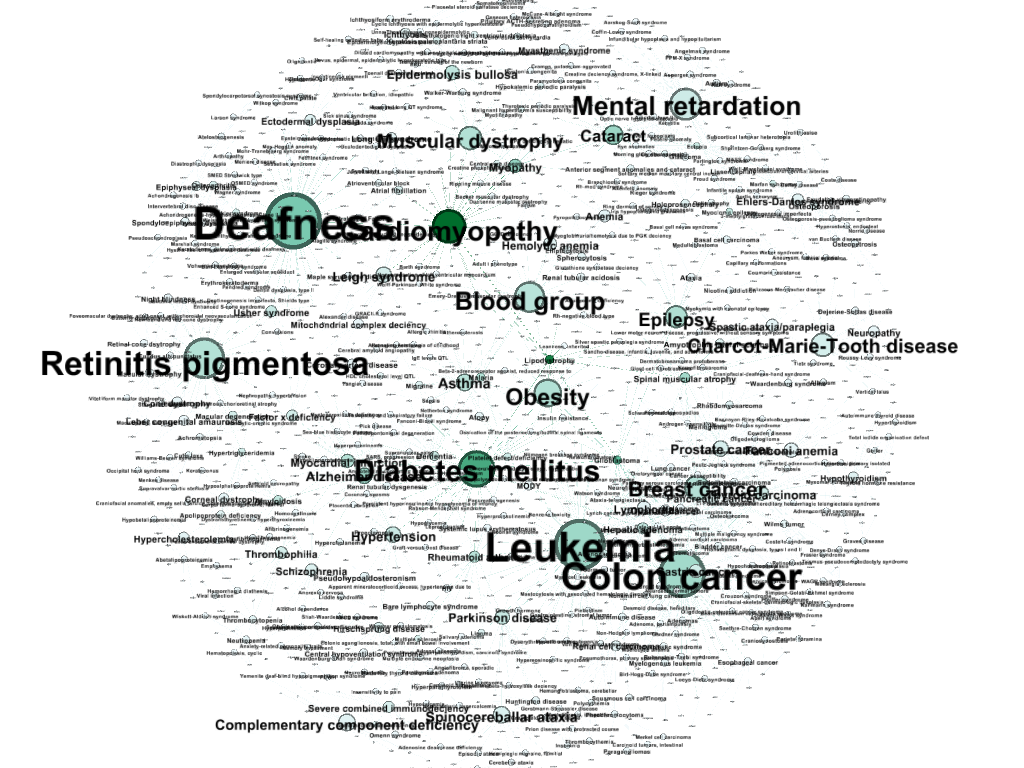
\includegraphics[width=0.75\textwidth]{images/Betweenness-Centrality}
	\caption{Centralidad de intermediación de la red completa.}
	\label{Betweenness-Centrality}
\end{figure}

\begin{figure}[H]
	\centering
	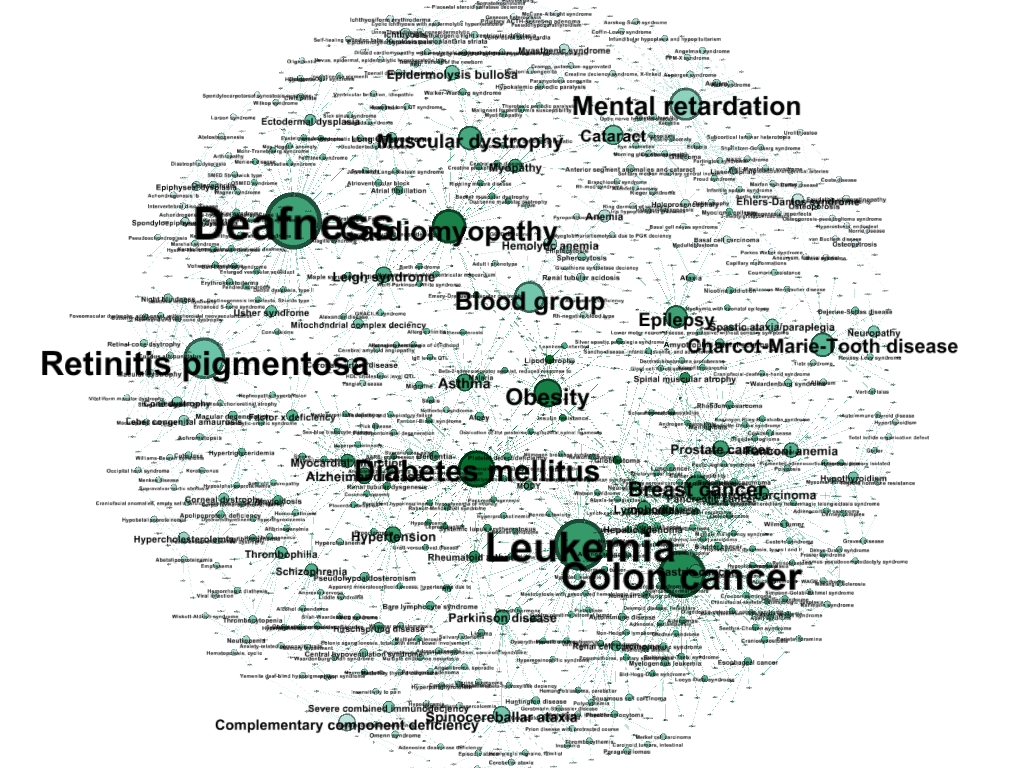
\includegraphics[width=0.75\textwidth]{images/Closeness-Centrality}
	\caption{Centralidad de cercanía de la red completa.}
	\label{Closeness-Centrality}
\end{figure}

\begin{figure}[H]
	\centering
	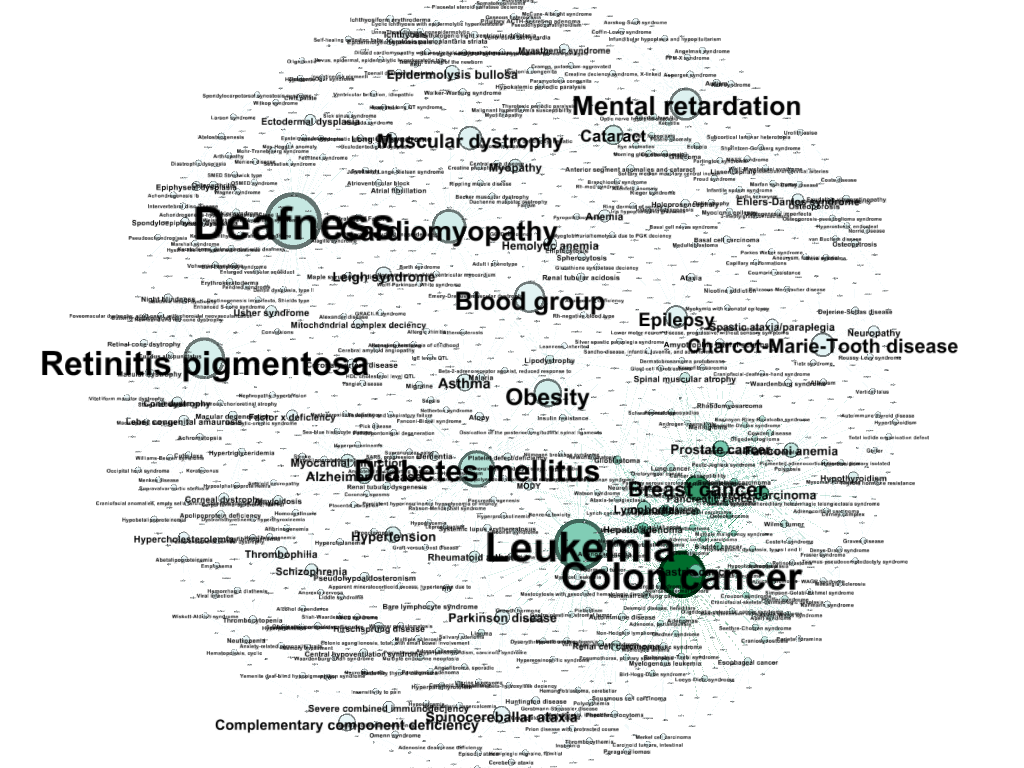
\includegraphics[width=0.75\textwidth]{images/Eigenvector-Centrality-Graph}
	\caption{Centralidad de vector propio de la red completa.}
	\label{Eigenvector-Centrality-Graph}
\end{figure}

\begin{figure}[H]
	\centering
	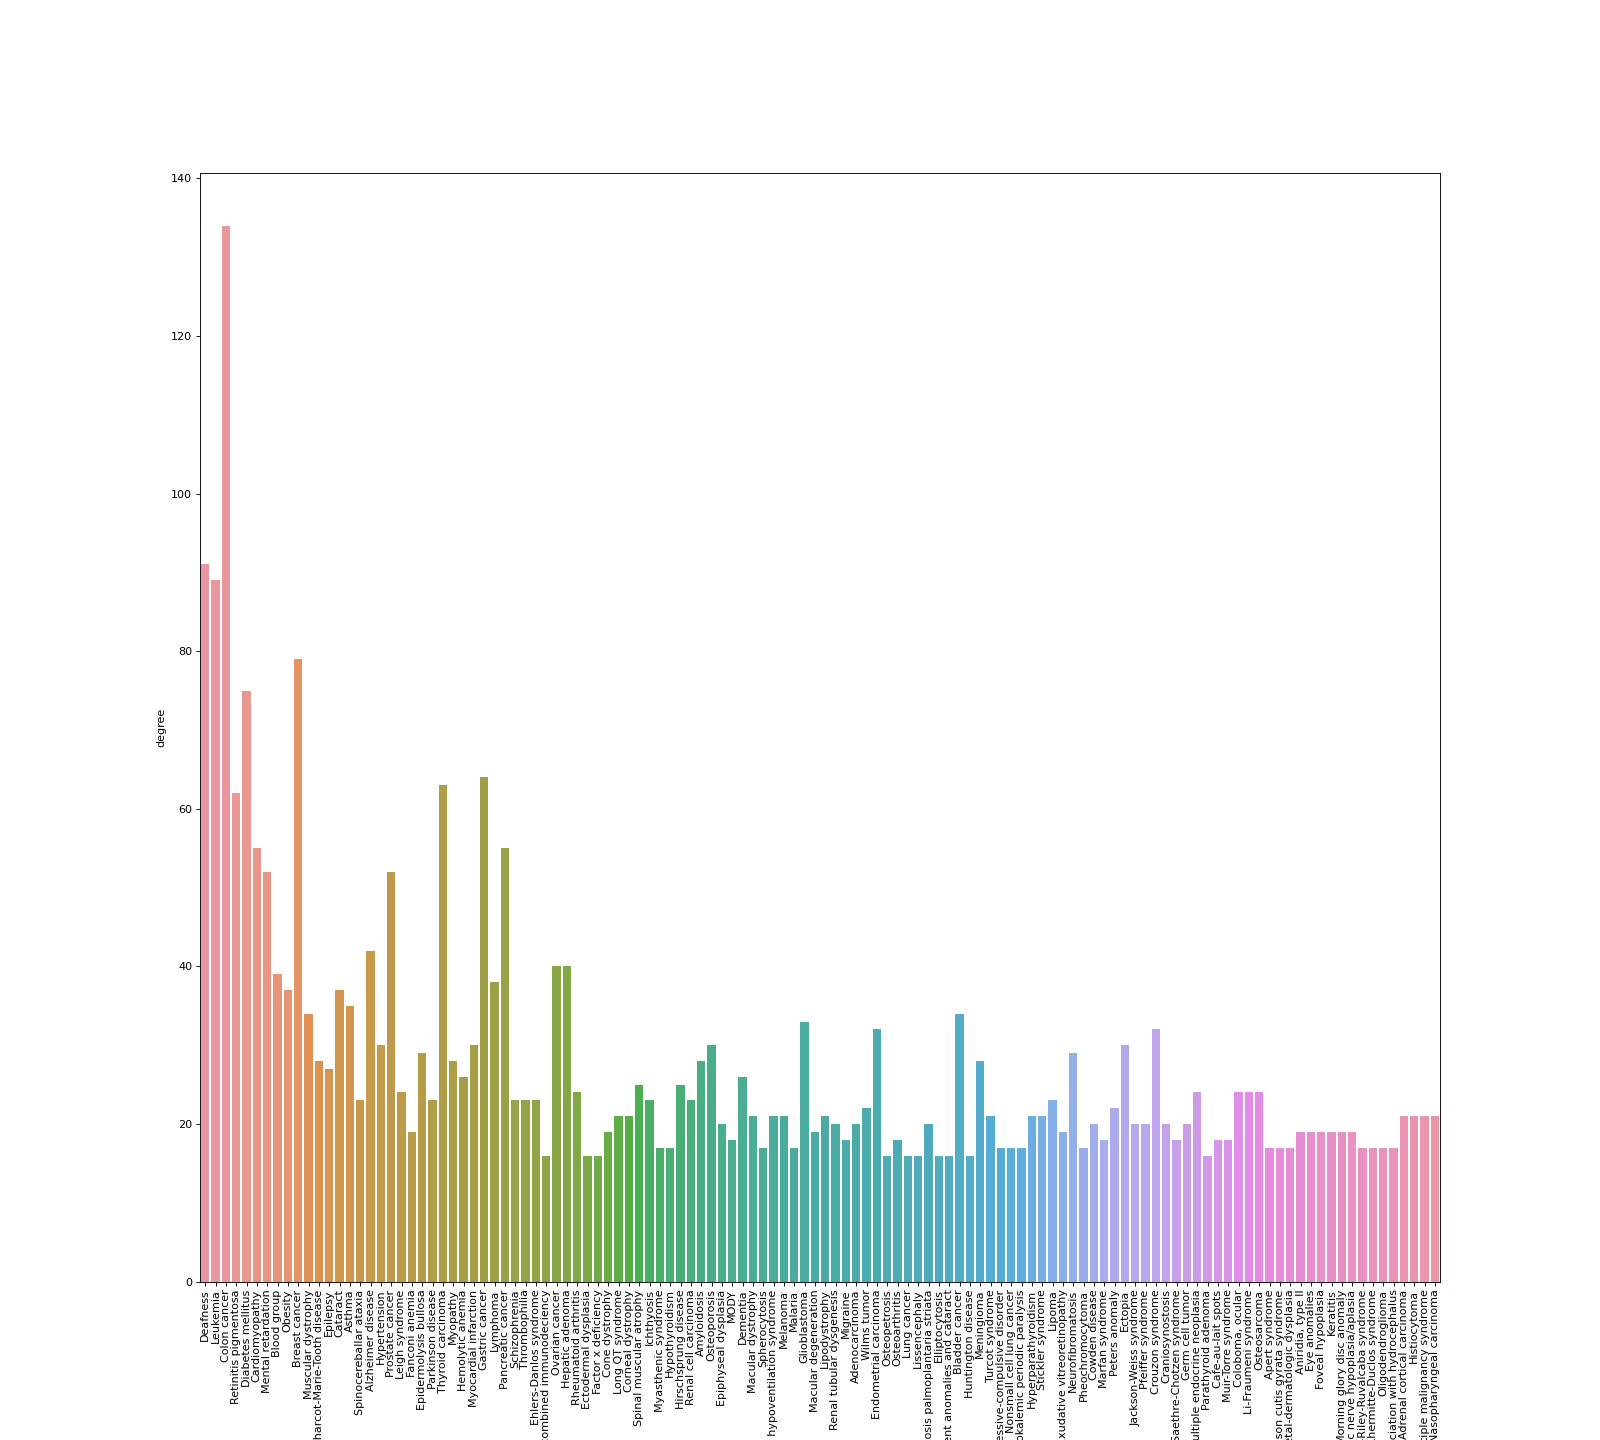
\includegraphics[width=0.65\textwidth]{images/degree}
	\caption{Actores de la medida de centralidad de grado.}
	\label{degree}
\end{figure}

\begin{figure}[H]
	\centering
	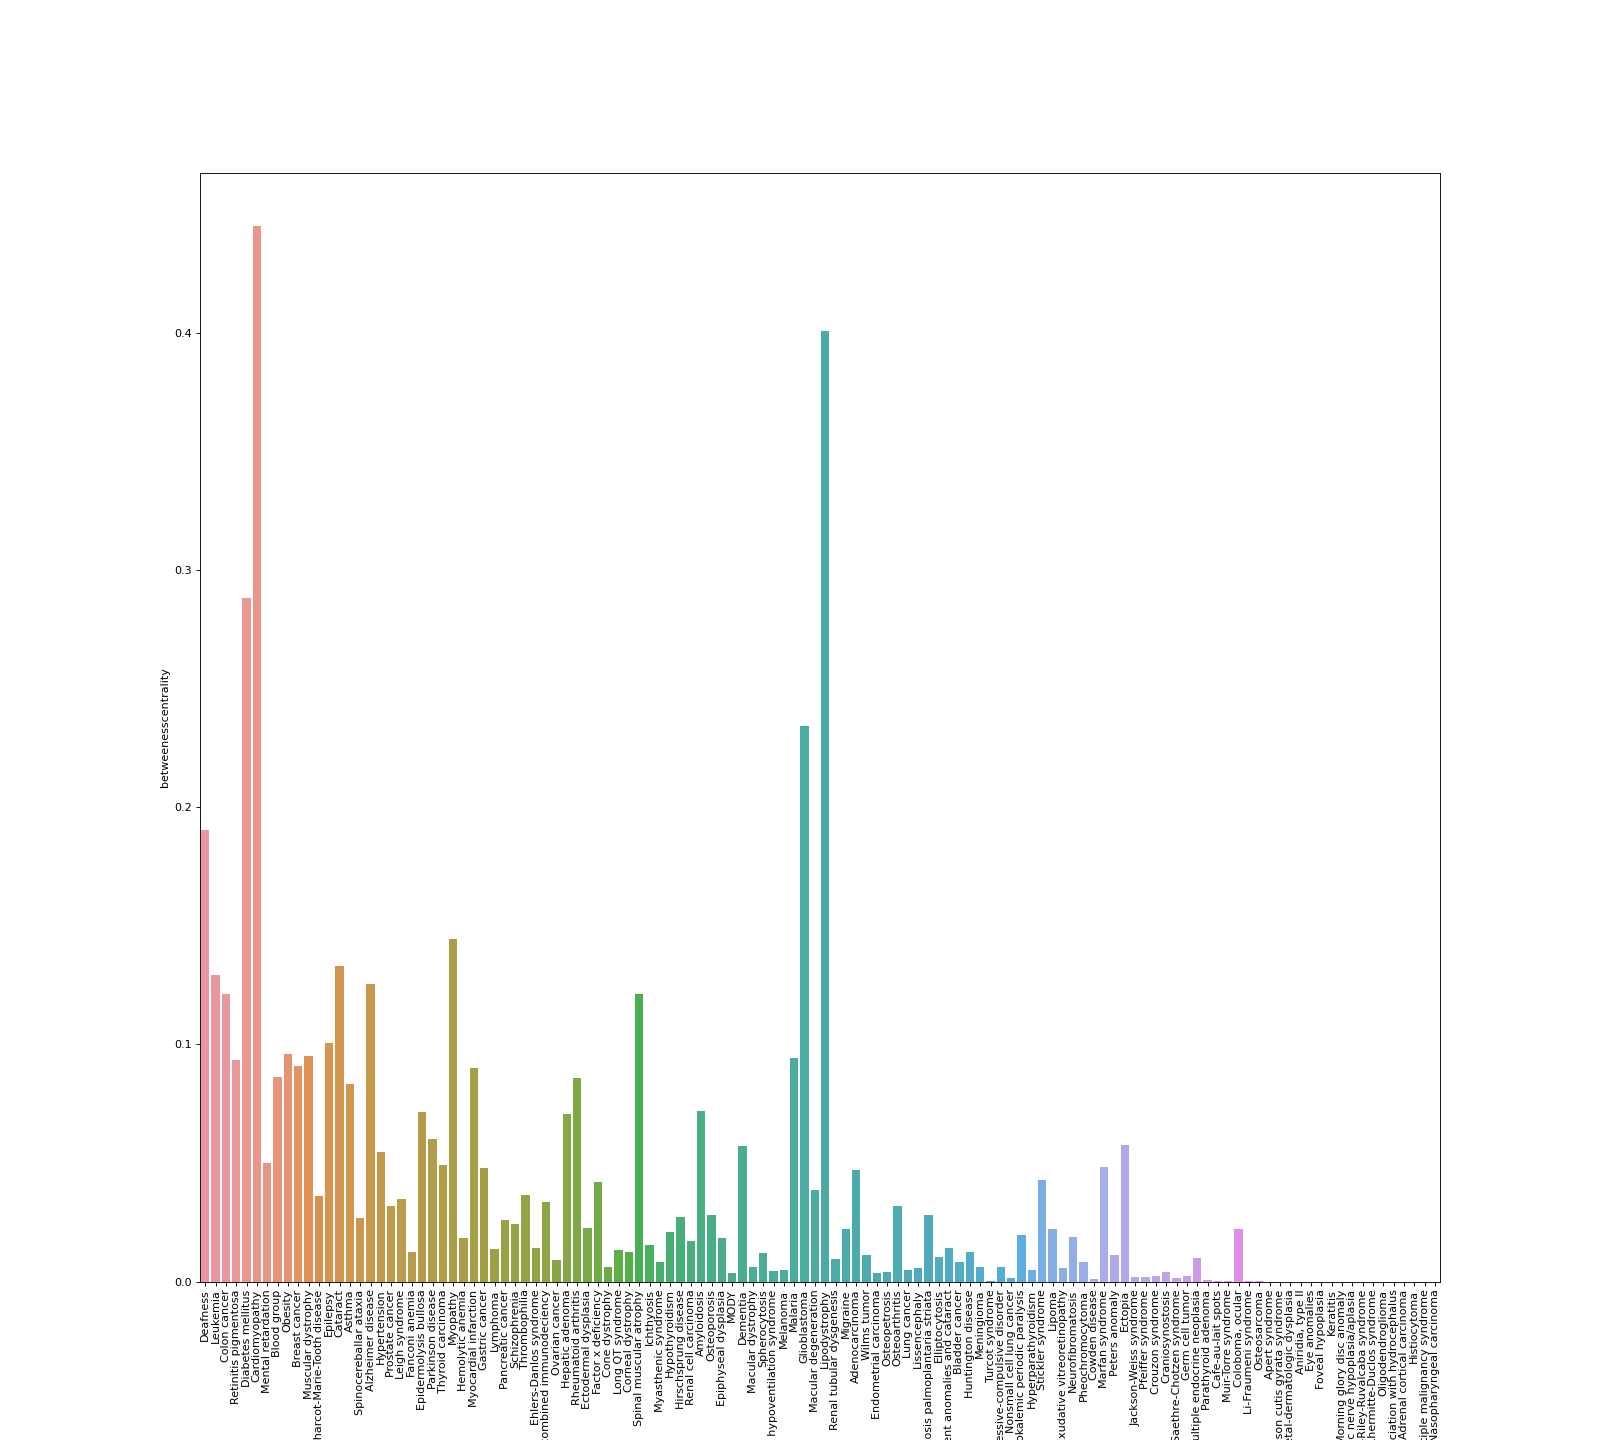
\includegraphics[width=0.65\textwidth]{images/betweenesscentrality}
	\caption{Actores de la medida de centralidad de intermediación.}
	\label{betweenesscentrality}
\end{figure}

\begin{figure}[H]
	\centering
	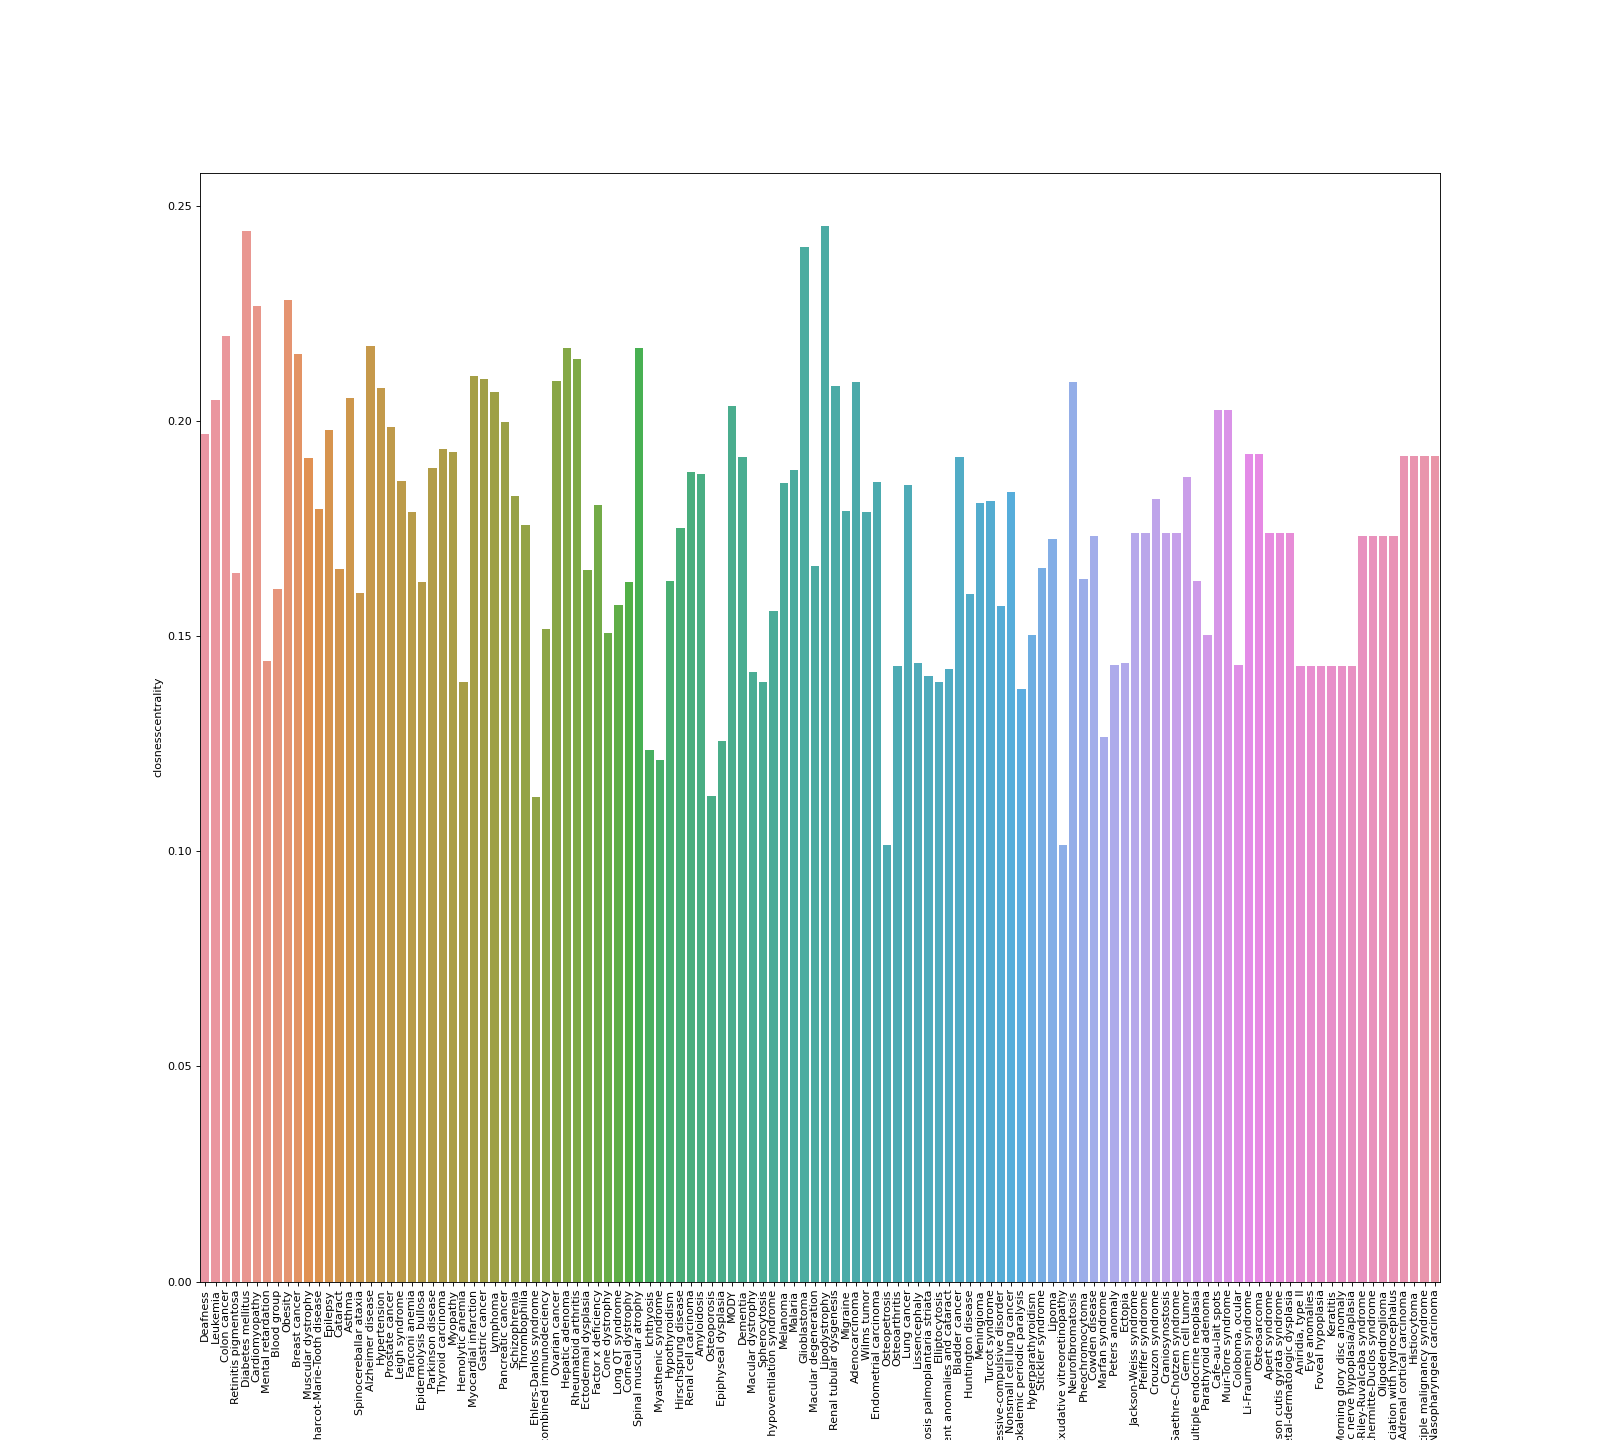
\includegraphics[width=0.65\textwidth]{images/closnesscentrality}
	\caption{Actores de la medida de centralidad de cercanía.}
	\label{closnesscentrality}
\end{figure}

\begin{figure}[H]
	\centering
	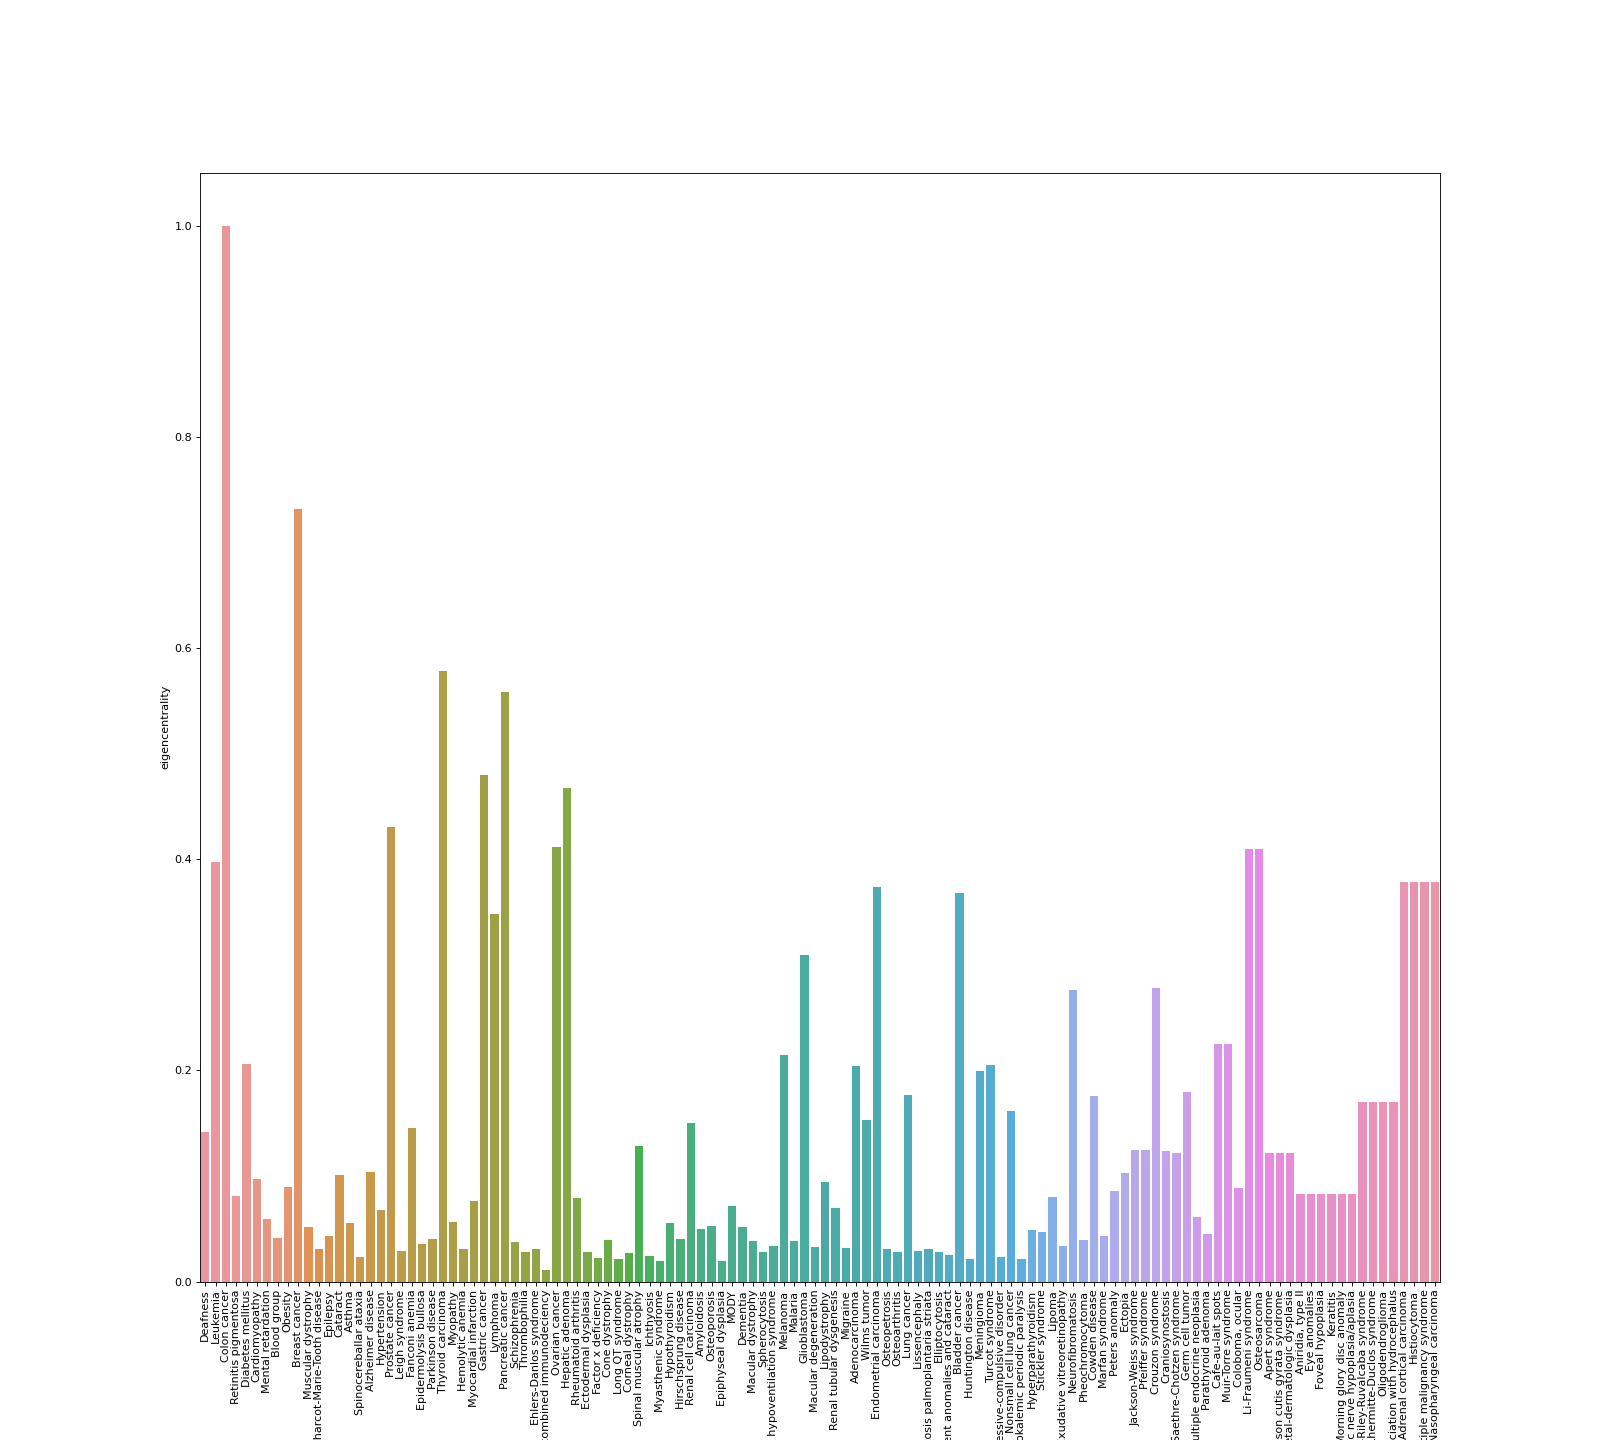
\includegraphics[width=0.65\textwidth]{images/eigencentrality}
	\caption{Actores de la medida de centralidad de vector propio.}
	\label{eigencentrality}
\end{figure}

Para realizar los gráficos anteriores, que representan los valores de las medidas para todos los actores de las enfermedades de la red en ejes de coordenadas, donde se han excluido algunas enfermedades y todos los genes, para poder mejorar las visualizaciones, se ha utilizado un \textit{script} en Python que se incluye en los ficheros de la práctica y que también podemos ver a continuación:

\begin{lstlisting}[language=Python, basicstyle=\small]
import seaborn as sns
import matplotlib.pyplot as plt
import pandas as pd


def createGraph(values, col):
	plt.figure(num=None, figsize=(20, 18), dpi=80, facecolor='w', edgecolor='r')
	g = sns.barplot(x="Label", y=col, data=values)
	plt.xticks(rotation=90)
	plt.savefig('images/{}.png'.format(col))


if __name__ == '__main__':
	df = pd.read_csv("dataset/diseasome.csv", sep=",")
	df_disease = df[df['0'].str.contains("disease")]
	df_disease = df_disease[df_disease["degree"] > 15]
	
	colNames = ["degree", "betweenesscentrality", "closnesscentrality", "eigencentrality"]
	for colName in colNames:
		createGraph(df_disease, colName)
\end{lstlisting}

\newpage

\renewcommand{\refname}{Bibliografía}
\bibliographystyle{unsrt}
\bibliography{biblio}

\end{document}
